\section{Motor control}
The motor controller should keep the speed of the motor consistent.
In order to ensure this, a PI controller is implemented to keep the speed constant of 30 rps.
The motor does not have inbuilt encoders, so in order to get some feedback for the controller, 3 Hall effect sensors are implemented.
A ramp up function is also implemented.

\subsection{Controller}

To ensure a smooth picture the PCB should rotate at a constant speed.
This is done using a PI controller, with a gain that is not too big since overshoot is not desirable and an integrator in order to reduce the steady state error.

\subsection{Encoders} \label{sec:encoders}

Hall effect sensors responds to magnetic fields.
By mounting a magnet in the rotating board, the Hall sensors will respond when the board is above the sensors, indicating where the board is.
In order to calculate the current speed of the rotating pcb, 3 Hall effect sensors are mounted on the board located under the rotating PCB.
The Hall sensors have been equally distributed with $120^{\circ}$ between them.

In order to get a binary from the analog Hall effect sensor, a Schmitt trigger\cite[p. 655]{book:prac_ele} is added on the output of the Hall effect sensor.
It is worth noting that the supply voltage is for the Hall effect sensor is 5V, which means that the output will be between 0 and 5 V, making the Schmitt trigger, go from 0 to 5 V.
The problem with this is that the FPGA cannot handle 5V, since it is a 3.3 V device.
This can be fixed by using a logic level converter. 

The for the logic level converter 

The speed is can be calculated by counting up a counter between getting logic high from one of the Hall effect sensors to  logic high on one of the others, using equations  \ref{eq:calc_time} and \ref{eq:calc_speed}.

\begin{equation} \label{eq:calc_time}
 t = \frac{20\cdot \text{counter}}{1\cdot 10^9}
\end{equation}

\begin{equation} \label{eq:calc_speed}
 \text{speed} = \frac{1}{3\cdot t}
\end{equation}

\subsubsection{Schmitt Trigger}
A Schmitt trigger is a common amplifier circuit with positive feedback to create hysteresis, so when the input to the Schmitt trigger goes over a specific threshold, the output goes high, and when the input goes under a different, lower threshold, the output goes low.
The choice of using a Schmitt trigger instead of a standard comparator is to reduce sensor noise when the magnet is moving over the sensor.
This ensures the signal goes high when the magnet approaches and not going below before the magnet has left.

\subsubsection{Schmitt trigger calibration} \label{sec:schmitt_cal}
In order to find at what the hysteresis voltages, a test was done on the output of the Hall effect sensor as function of distance from sensor.
The test was done by moving a magnet over the Hall effect sensor, so the Hall effect sensor is gradually covered and uncovered again. The magnet was kept at the height over the Hall effect sensor that it would have in the final product, 2 mm. 
The result can be seen in figure \ref{fig:hall_out}.

\begin{figure}[h]
 \centering
 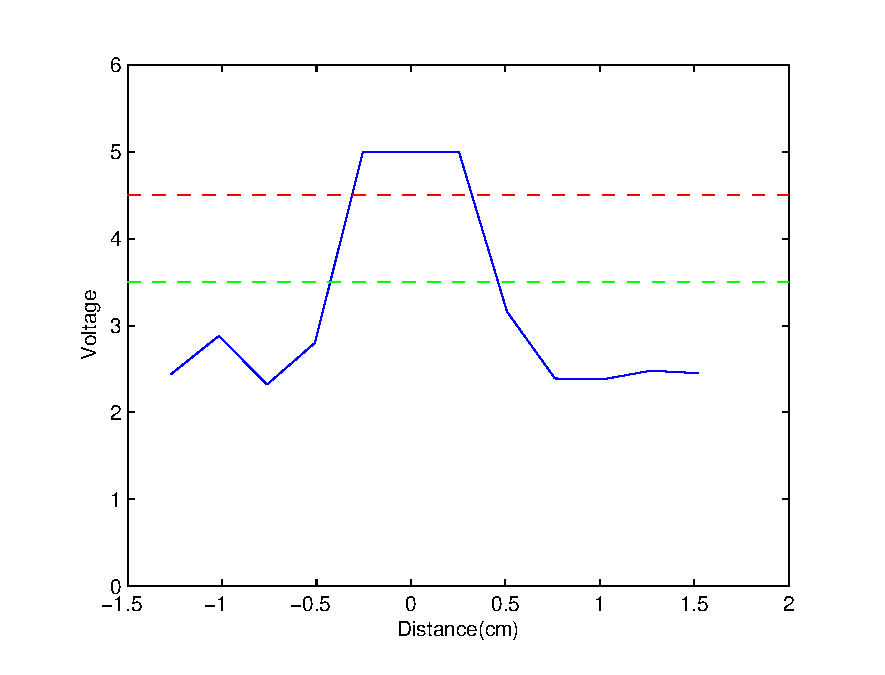
\includegraphics[width=0.6\textwidth]{img/hall_out}
 \caption{Output of the Hall effect sensor as function of distance from the sensor. The dashed lines represent where the hysteresis thresholds lie.}
 \label{fig:hall_out}
\end{figure}

From figure \ref{fig:hall_out} the low and high hysteresis thresholds are chosen to be 4.5 V for the high, and 3.5 V for the low threshold.

\subsection{Ramp up}

The ramp up function is implemented to get a faster speed up time.
If this is not implemented, either an aggressive controller has to be implemented for the entire system, which is not desirable, or the time to reach the desired speed will become very long.

Instead of this, another controller is implemented, which is basically just an integrator.
When the integrator reaches a specified speed, the regular controller takes over. 


\subsection{Driving the motor}

The motor, a normal dc motor, is controlled using pulse width modulation (PWM). The duty cycle is calculated by the controllers as seen in equation \ref{eq:duty}. The maximum speed is defined by the gearing of the motor, and the max RPS at the given voltage, see datasheet \cite{datasheet:motor}. 

\begin{equation}\label{eq:duty}
 \text{duty} = \frac{\text{output}}{\text{max\_speed}}\cdot 100 = \frac{\text{output}}{100\cdot \text{gearing\_ratio}}\cdot 100
\end{equation}

The PWM output is put out on an I/O pin and fed into a mosfet capable of sourcing enough current.
A NTD5867NL MOSFET is chosen for this since it can source up to 20 A\cite{datasheet:mosfet} and is available in the component storage.
